% Definition du répertoire contenant les images
\graphicspath{{IMAGE/}}

% FRAME Intro
\begin{frame}
%TODO logos

\includegraphics[width=12cm]{Logos.pdf}

\vfill

\begin{center}

\vspace*{1.5cm}

\LARGE
\textbf{Geographic Information}

\vspace*{1.5cm}
 DELHI GIS-R School


\large
9-12\up{th} April 2019

\vspace*{1.5cm}


\textbf{Hadrien Commenges \& Paul Chapron}

{\small

\vspace*{0.1cm}

\url{hadrien.commenges@univ-paris1.fr}

\url{paul.chapron@ign.fr}

}

\end{center}

\end{frame}


% FRAME 
\begin{frame}{Definitions}

\begin{block}{Geographical Information }

Quantitative information, localized in 1, 2, 3 or n dimensions. 
This information is addressed from itls localization point of view.
\end{block}

~

\textbf{Geographical information types:}

\begin{enumerate}
\item Geographical objects (volcanos, railways, forest, etc.)
\item Event occurences (fires, crimes, etc.)
\item Measure points (altitude, temperature, etc.)
\item « Statistics » (population, unemployment rate, etc.)
\item Interaction measures (flows, catchment area, etc.)
\end{enumerate}

\end{frame}



% FRAME 
\begin{frame}{Definitions}

\begin{block}{The question of nature}
The nature of the geographical information is independent from the geographical object, 
 it has to be set by the analyst, according to the research question.
\end{block}

~

\begin{enumerate}
\item Dwellings point patterns (spatial object)
\item Dwellings sales (occurrences)
\item Dwellings prices (measure points)
\item Average price by district (« statistics »)
\end{enumerate}

\end{frame}



% FRAME
\begin{frame}{(1) Geographical Objects }

 Geographical objects come in three types : \textbf{points}, \textbf{lines} and \textbf{areas}. Geographical data analysis focus on their \textbf{geometry} (e.g. length, morphology) and their \textbf{topology} (e.g. neighborhood , distance).

\begin{figure}
  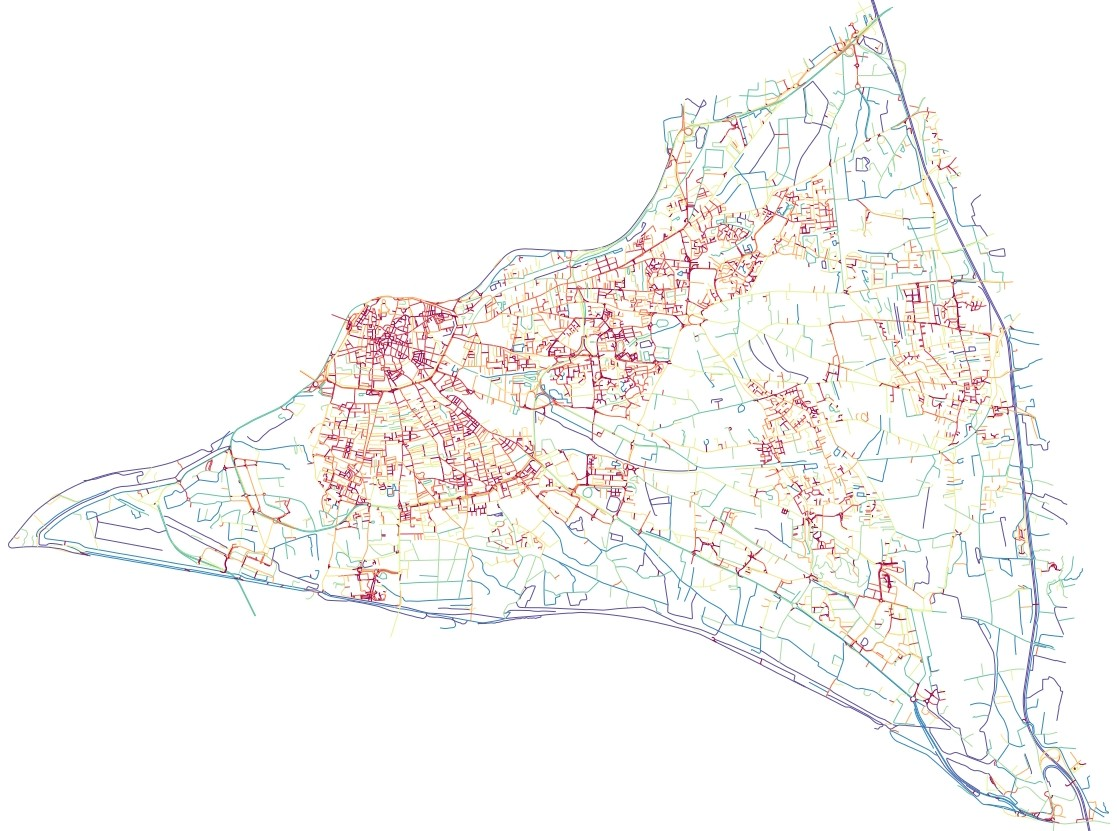
\includegraphics[width=8.5cm]{Morpheo.jpg}
\end{figure}

\end{frame}


% FRAME
\begin{frame}{(2) Event occurence}

 \textbf{Point data}, \textbf{sampled or extensive}, whose localization is under study. 
When it comes to model, localization is  the \textbf{response variable}.

\begin{figure}
  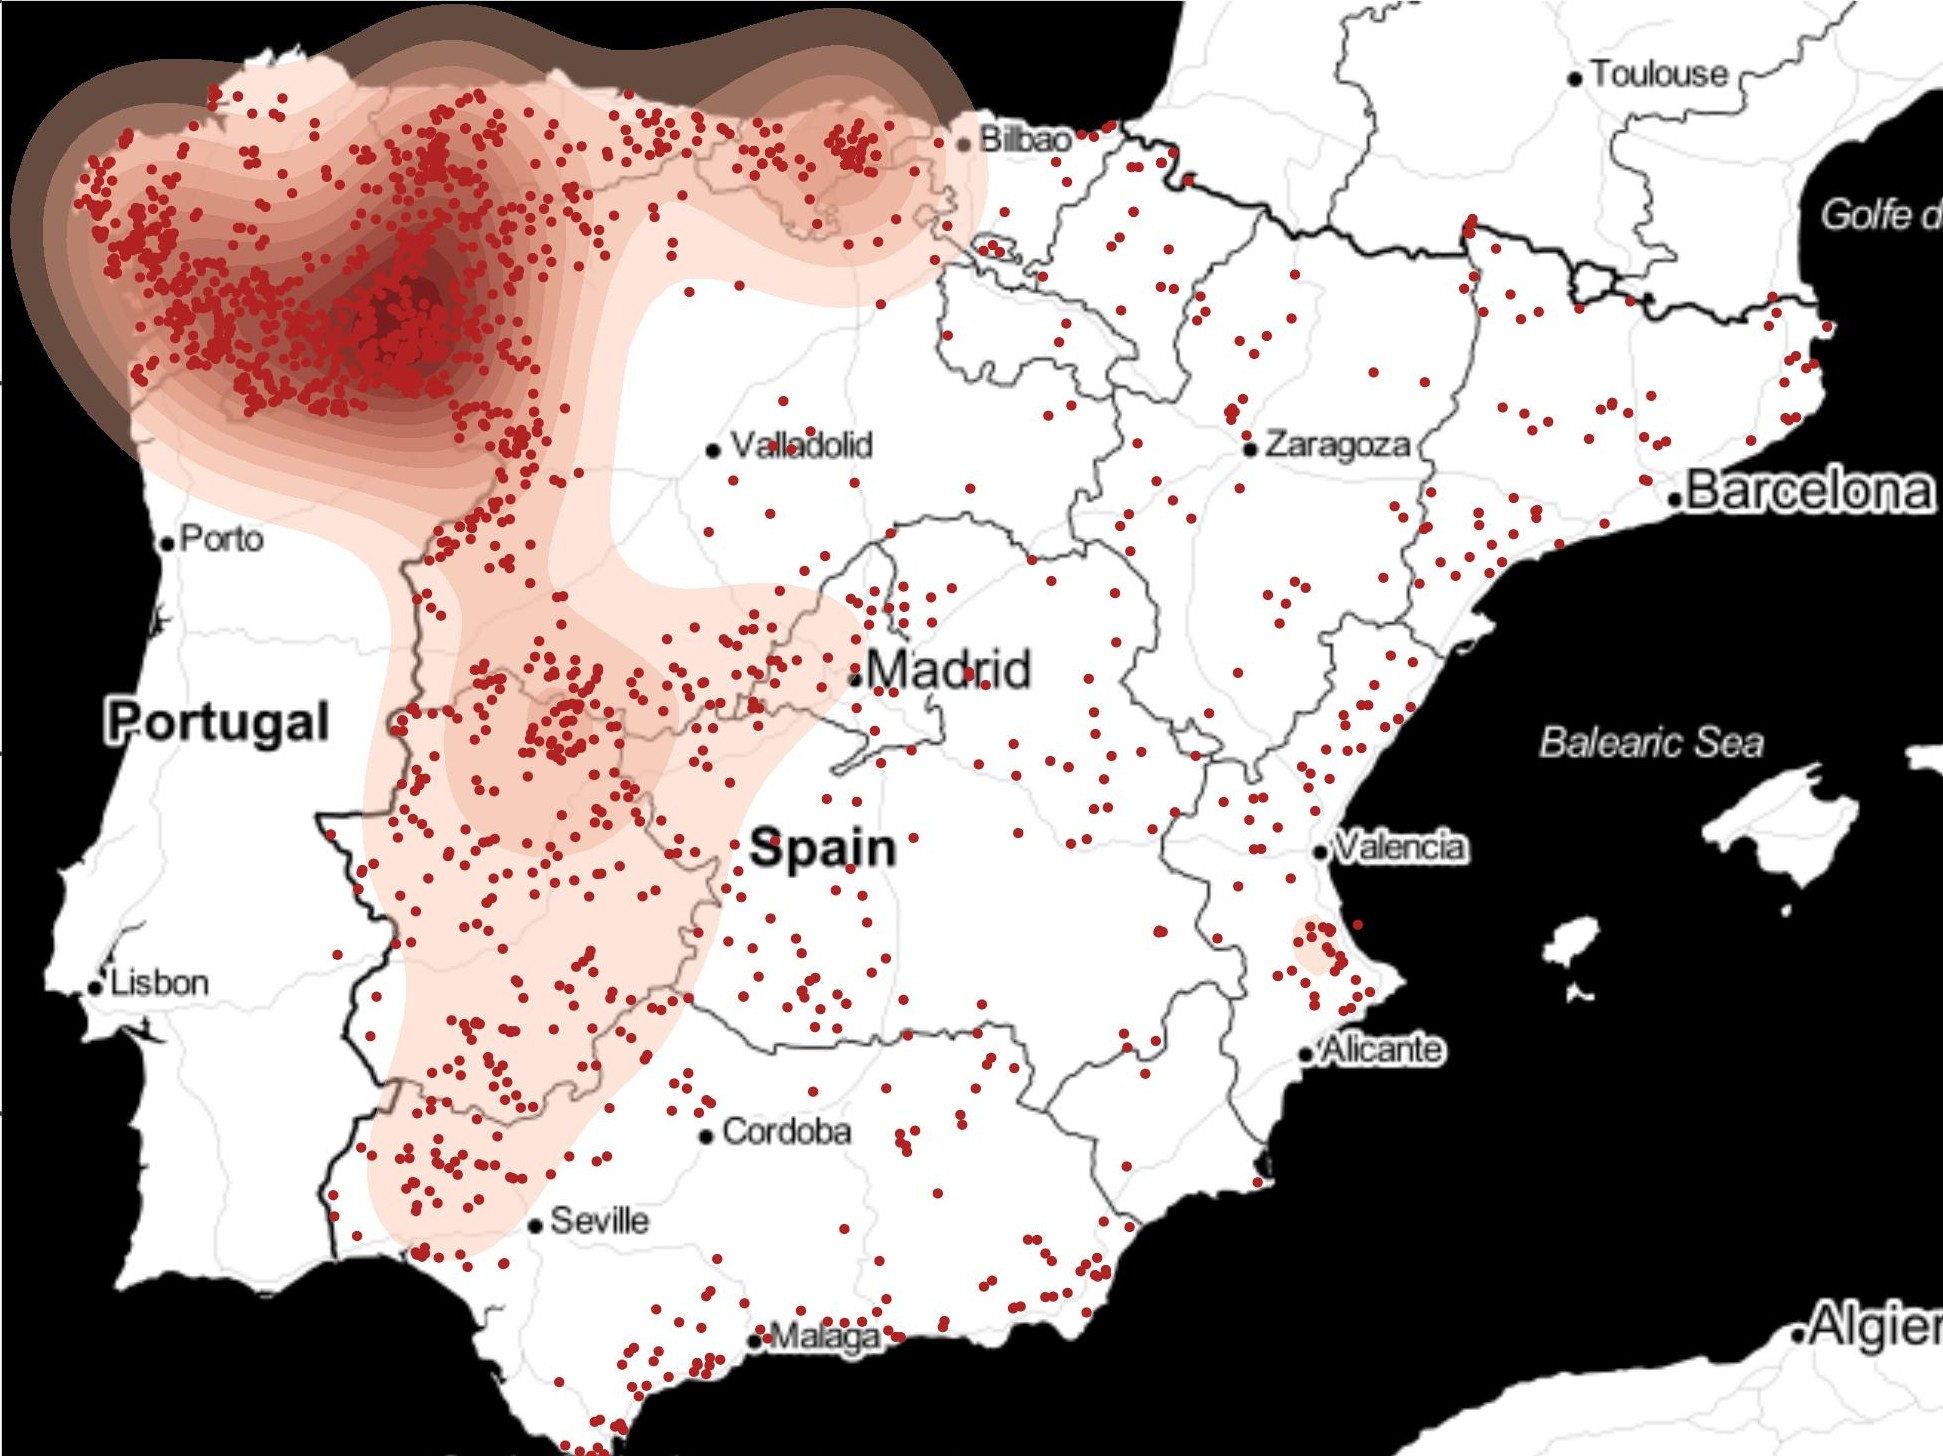
\includegraphics[width=8.5cm]{Incendies.jpg}
\end{figure}

\end{frame}


% FRAME
\begin{frame}{(3) Measure points}

 \textbf{Point data}, \textbf{sampled or extensive}, where a \textbf{value} is associated to each localization.  Phenomenon under study is \textbf{the value variation according to the localization}.

\begin{figure}
  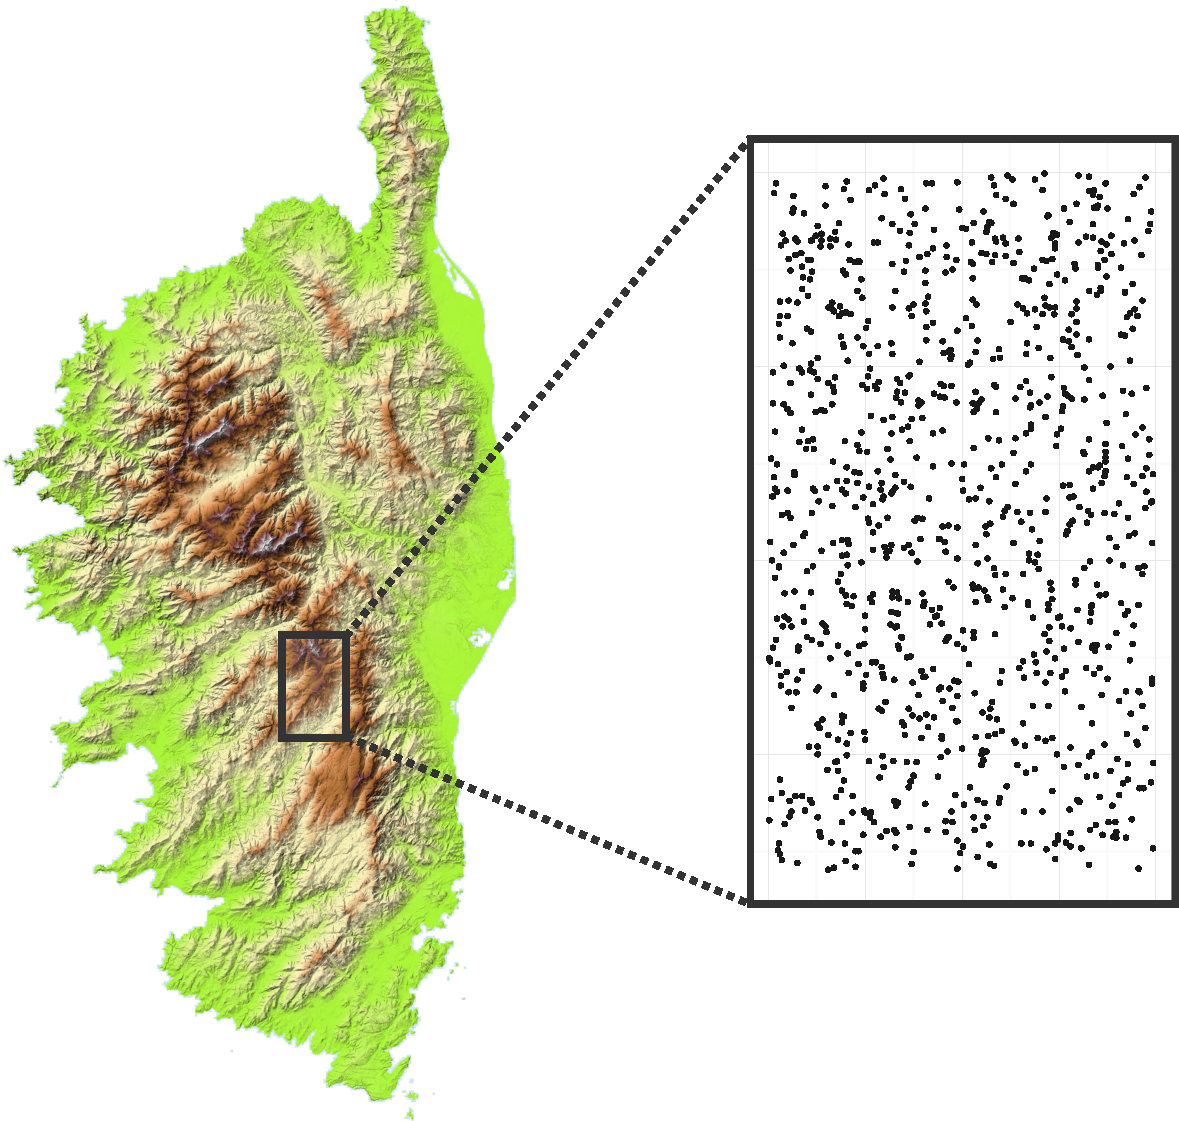
\includegraphics[width=6.5cm]{Corse.pdf}
\end{figure}

\end{frame}


% FRAME
\begin{frame}{(4) Statistics}

«Statistics», from \textit{statista}, «state man»  in italian. \\
\textbf{Zonal extent variables} created from census - \textbf{sampled or extensive} - for territorial management.

Such variables are attributes measured or computed \textbf{within spatial units}.

\begin{figure}
  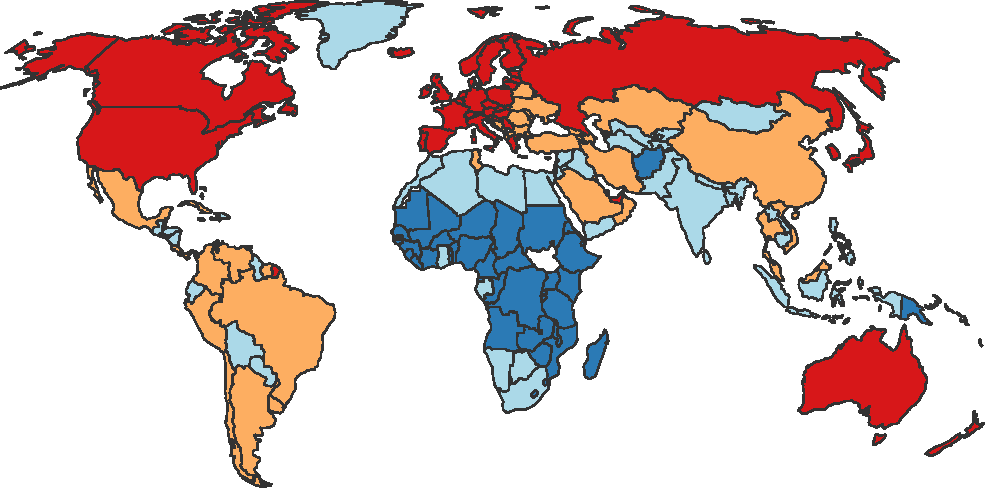
\includegraphics[width=10cm]{World.pdf}
\end{figure}

\end{frame}


% FRAME
\begin{frame}{(5) Interactions}

Interactions concern  \textbf{geographical objects},  \textbf{occurrences} or  \textbf{spatial units} and the \textbf{links} between them.
The object under study is the \textbf{structure} and \textbf{dynamic} of these links (network analysis).

\begin{figure}
  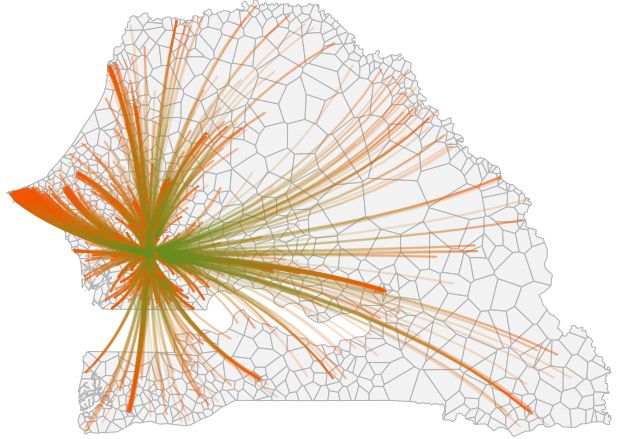
\includegraphics[width=8cm]{Interaction.png}
\end{figure}

\end{frame}




% FRAME
\begin{frame}{Coordinates, areas, distances}

 \textbf{Geolocation} of a spatial entity  depends on:

\begin{itemize}
  \item \textbf{Reference ellipsoid}: Clarke1880, Ellipsoide1909, IAG-GRS80
  \item \textbf{Geoid} : gravity field equipotential surface 
  \item \textbf{Projection}: Mercator, Lambert, Mollweide, etc.
\end{itemize}

 A \textbf{Geodetic system} (or datum) is the combination of these 3 elements (e.g. WGS84)

\end{frame}

% FRAME
\begin{frame}{Coordinates, areas, distances}

%TODO traduire image ?
\begin{figure}
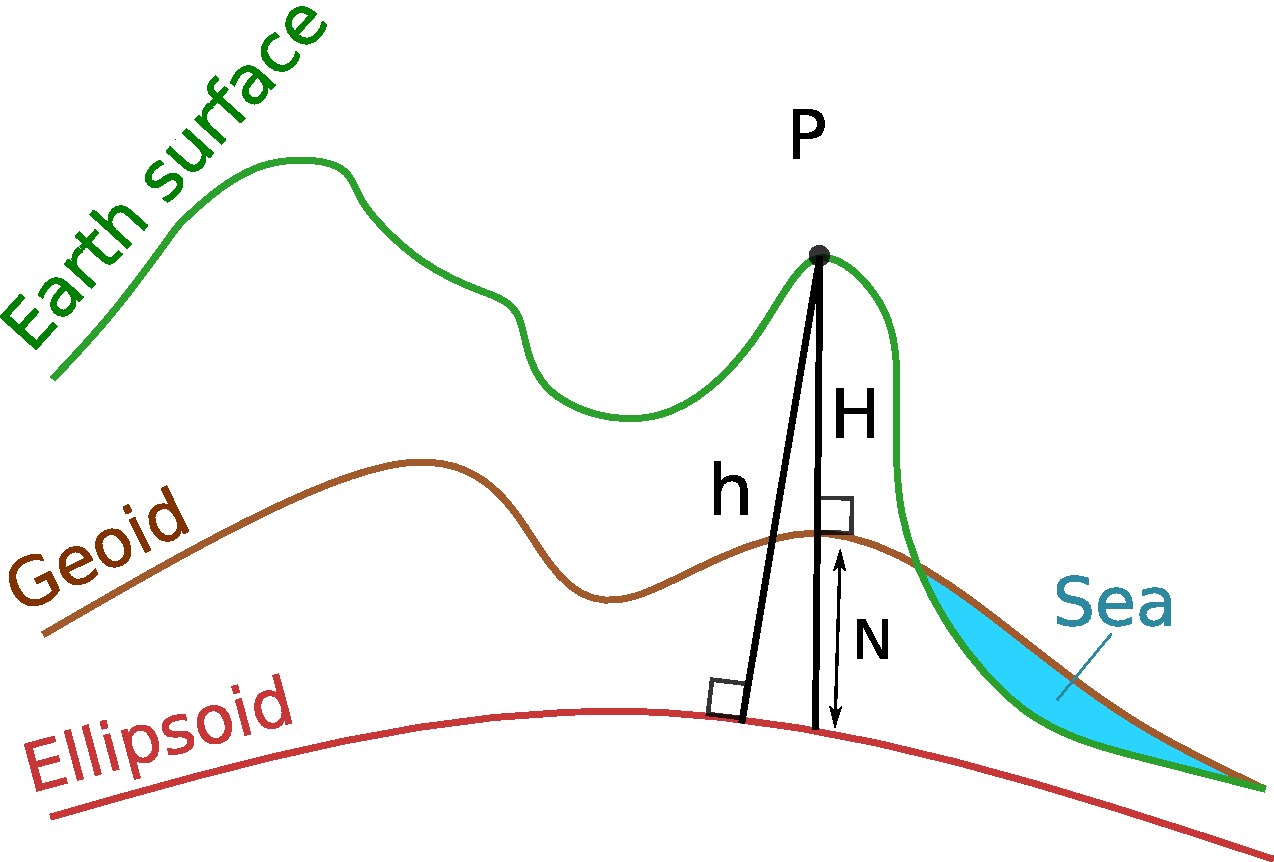
\includegraphics[width=9.5cm]{Geoide_EN.pdf}
\end{figure}

\footnotesize
\emph{Source: ENSG, Les projections et référentiels cartographiques}
\normalsize

\end{frame}



% FRAME
\begin{frame}{Coordinates, areas, distances}

\begin{figure}
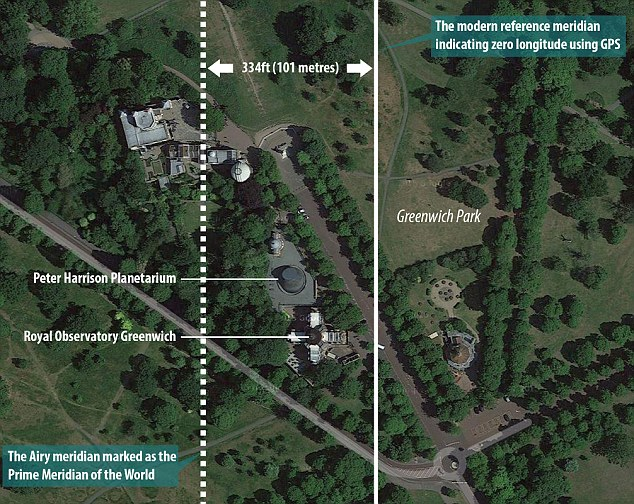
\includegraphics[width=9.5cm]{Greenwich.jpg}
\end{figure}

\end{frame}


% FRAME
\begin{frame}{Coordinates, areas, distances}

A sphere (globe) is a \textbf{non-developable} surface, i.e. cannot be represented as a plane (map) without \textbf{deformation}.

~

Some projections preserve some features  
\begin{itemize}
  \item \textbf{conformal}: conserve angles (shape)
  \item \textbf{equivalent}: conserve areas
  \item \textbf{equidistant}: conserve distances
\end{itemize}

Some others don't. 

~

UTM (Universal Transverse Mercator, conformal) allows almost everywhere an acceptable projection. 

What is the recommandation for India ? Specific ? Kalianpur 5 zones ? 

\end{frame}


% FRAME
\begin{frame}{Coordinates, areas, distances}

\begin{figure}
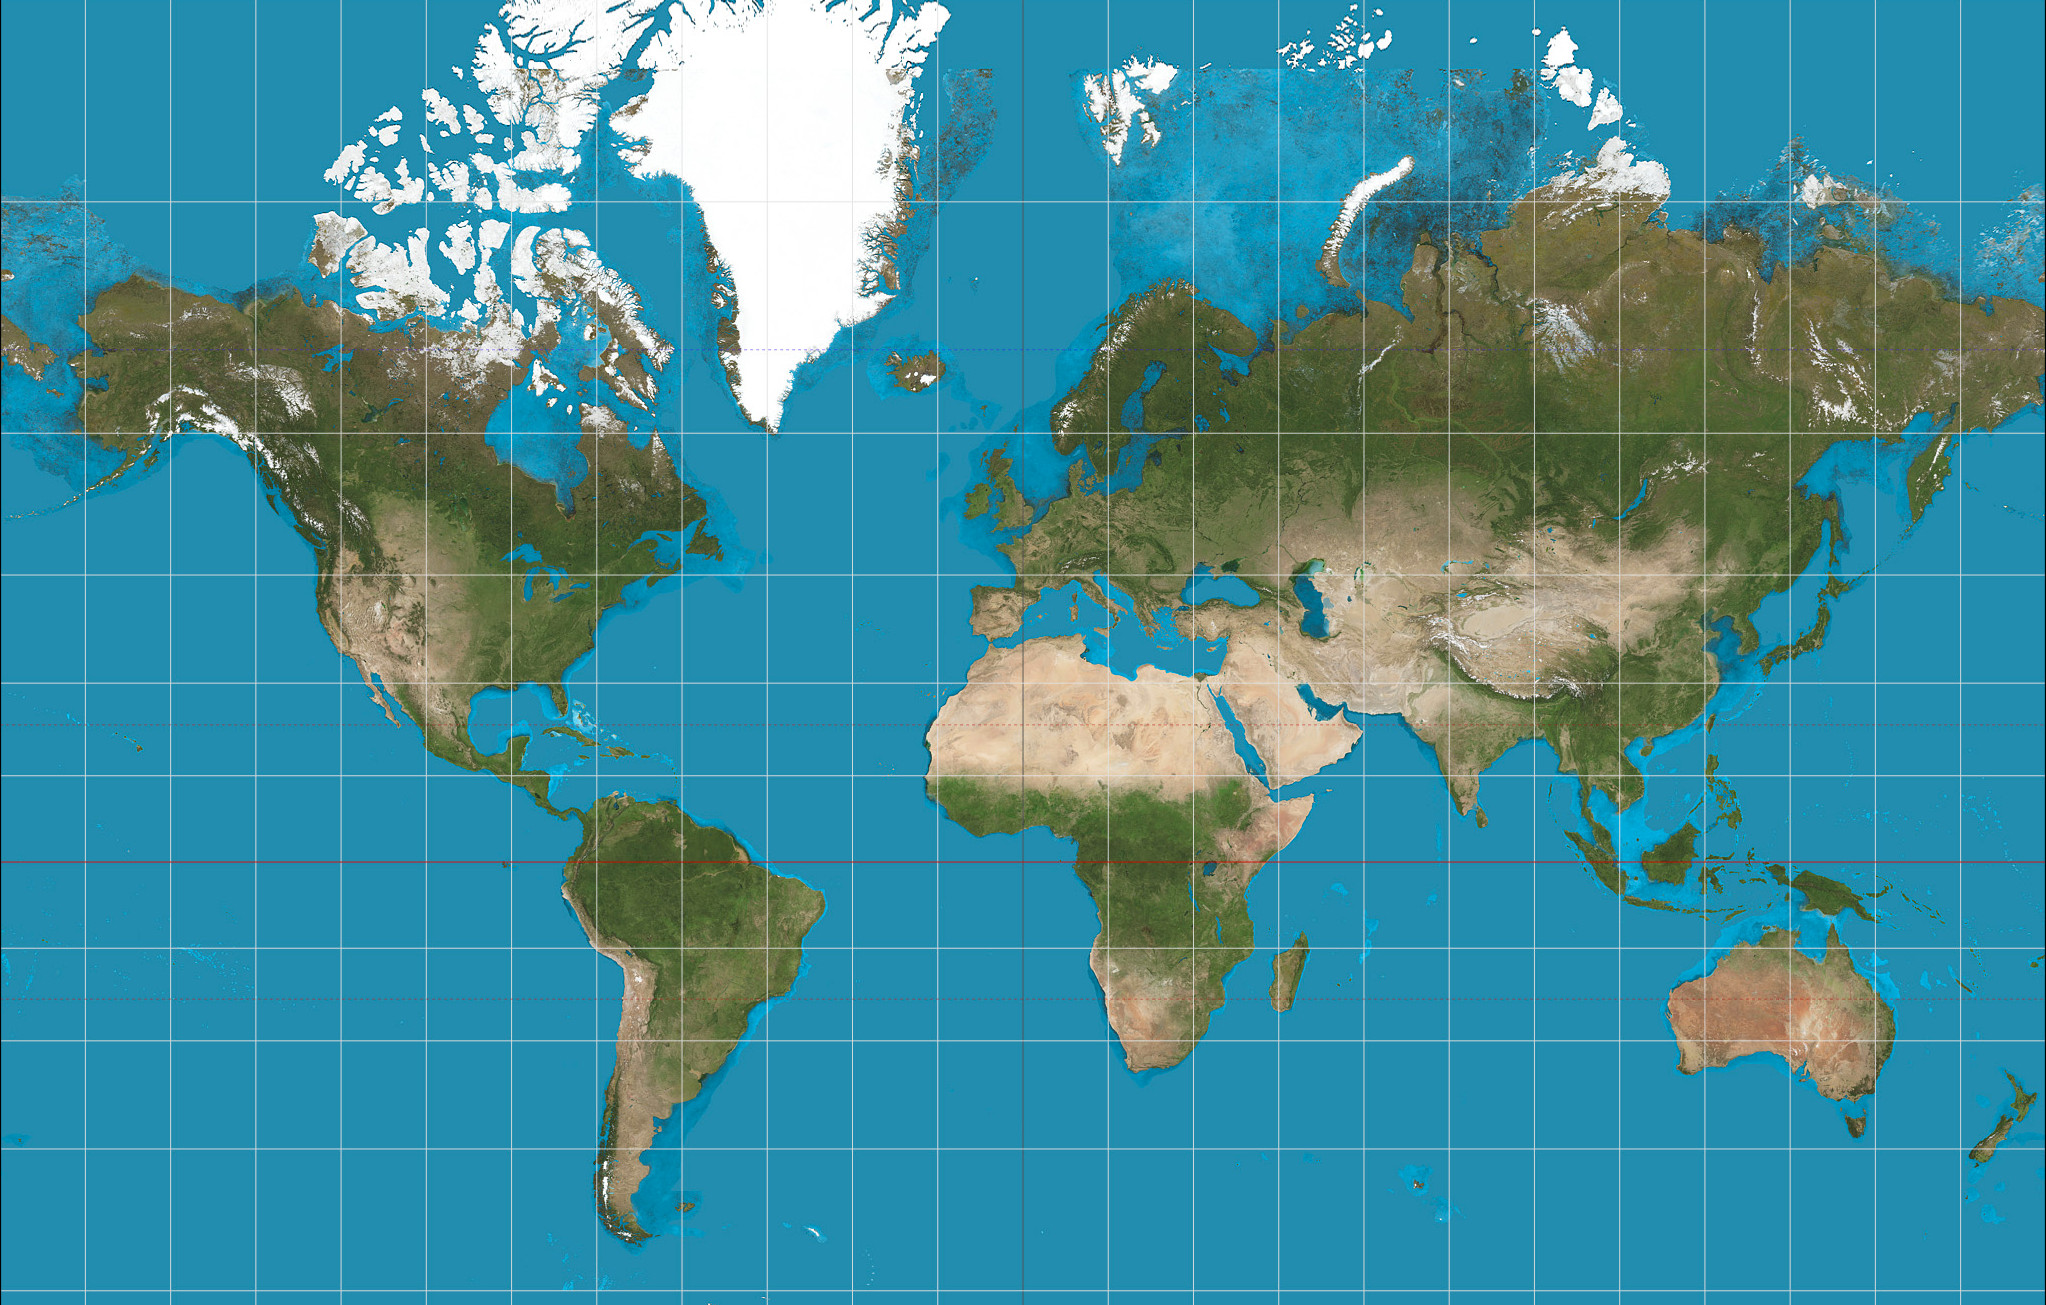
\includegraphics[width=11cm]{MercatorProj.jpg}
\end{figure}

\footnotesize
\emph{Source: Wikimedia, Mercator projection}
\normalsize

\end{frame}


% FRAME
\begin{frame}{Coordinates, areas, distances}

\begin{figure}
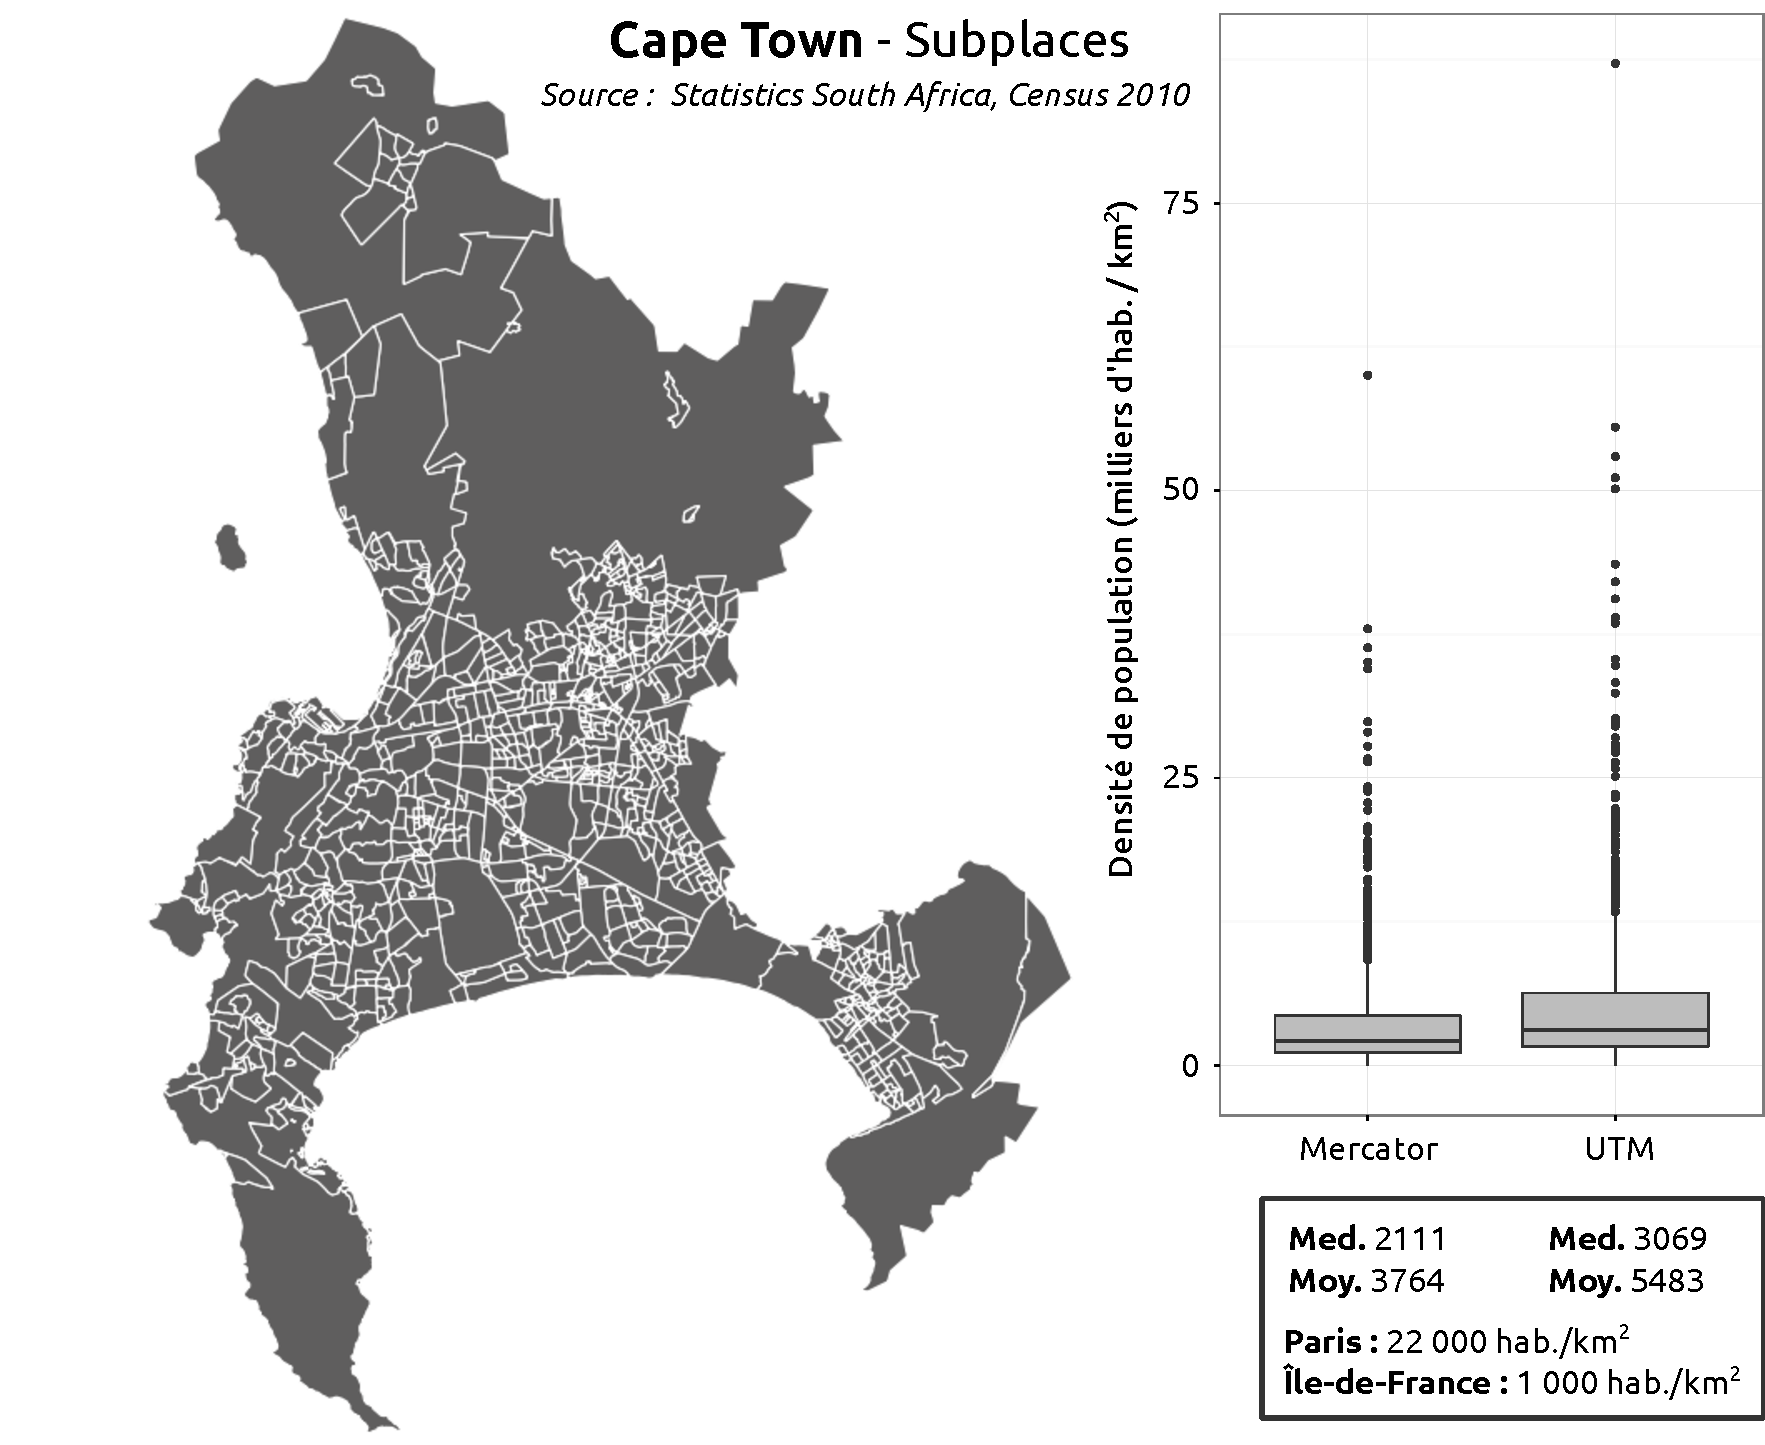
\includegraphics[width=9.5cm]{Projection.pdf}
\end{figure}

\end{frame}


% FRAME
\begin{frame}{Coordinates, areas, distances}

\begin{figure}
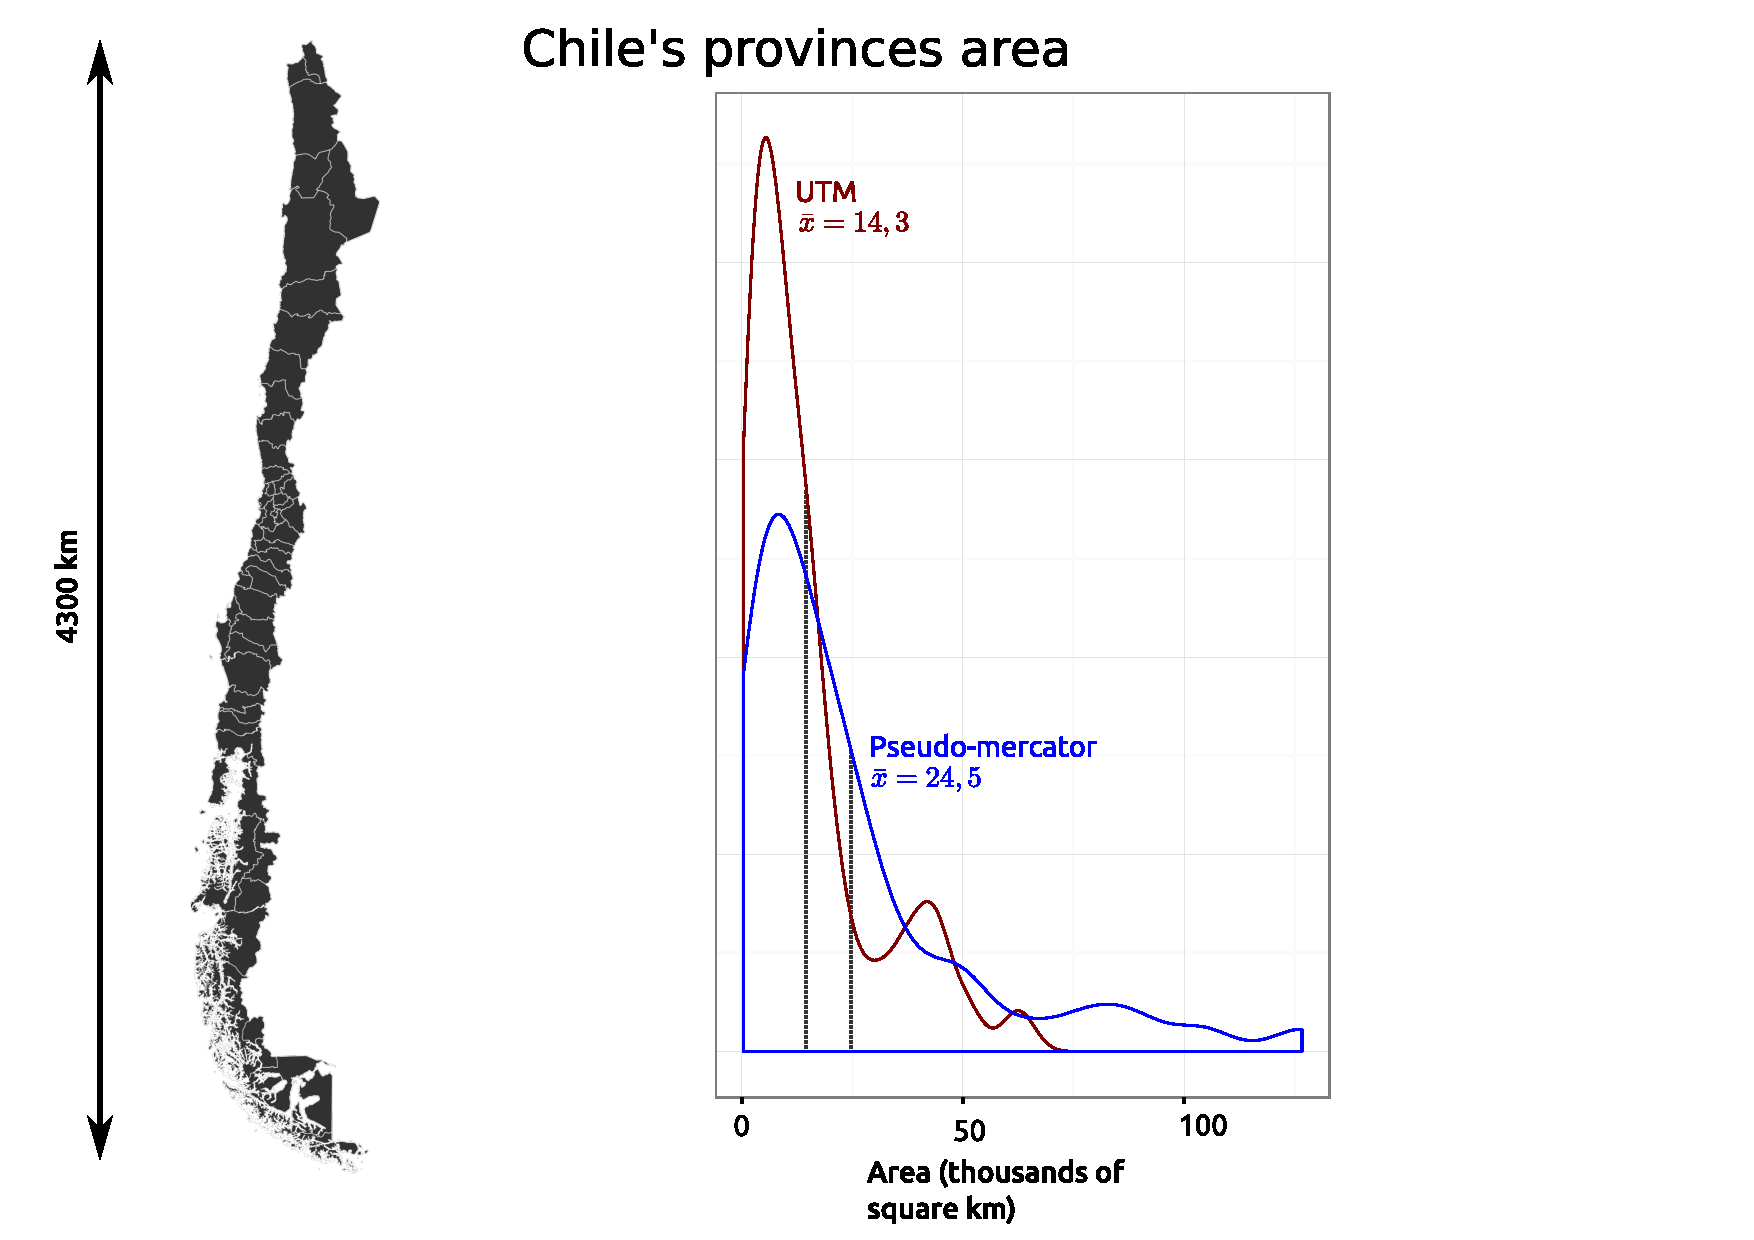
\includegraphics[width=10cm]{ChiliAire_EN.pdf}
\end{figure}

\end{frame}


% FRAME
\begin{frame}{Coordinates, areas, distances}

Basic precautions regarding projection : 

\begin{itemize}
  \item Density $\rightarrow$ any areas alteration ? 
  \item Distance $\rightarrow$ any length alteration ? 
\end{itemize}

~
Regarding  measures :   It depends on the scale ! (and the devices)  

~

GPS-RTK (centimetric precision) or Great-circle distance ? 

\begin{figure}
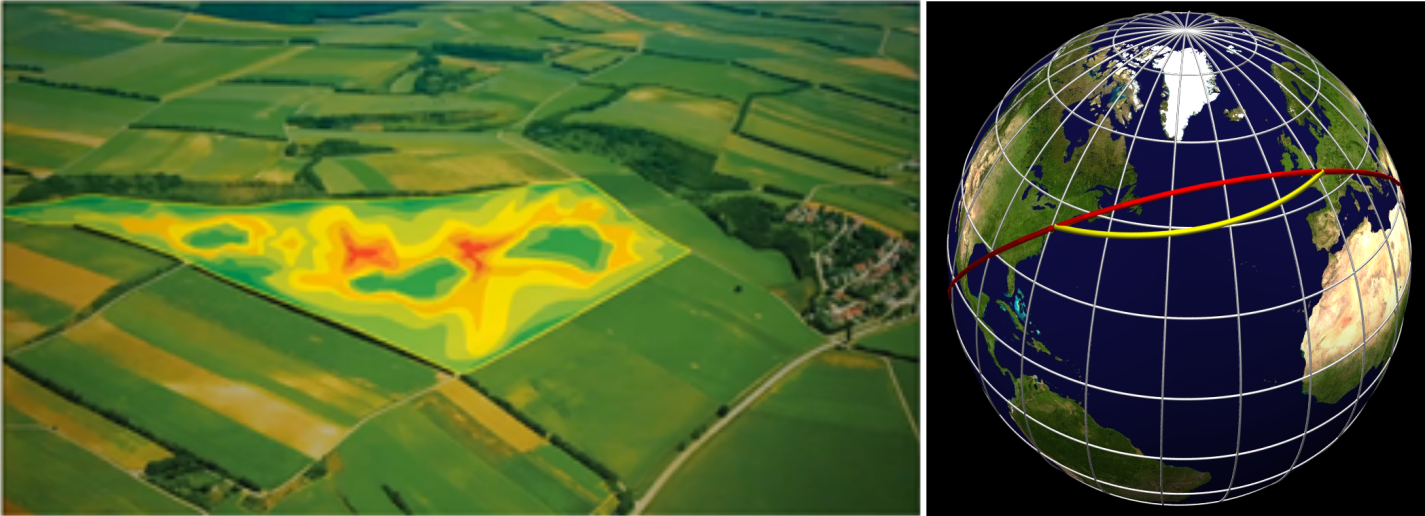
\includegraphics[width=10cm]{Echelle.png}
\end{figure}

\end{frame}


% FRAME
\begin{frame}{Modeling and representation}

\begin{small}
\textbf{to model} (here), is defining \textbf{categories} of objects \textbf{depicting} real-world objects (somehow linked to ontologies).
\end{small}

\begin{figure}
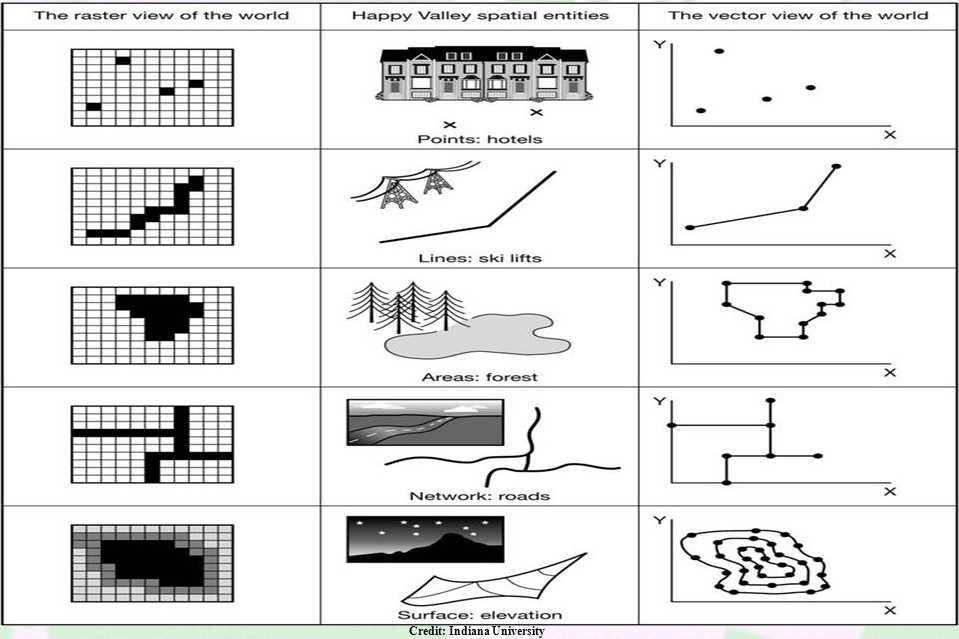
\includegraphics[width=10.5cm]{RasterVector.jpg}
\end{figure}

\end{frame}




% FRAME
\begin{frame}{Modeling and representation}
\textbf{Objects} and  \textbf{Fields}.

\begin{figure}
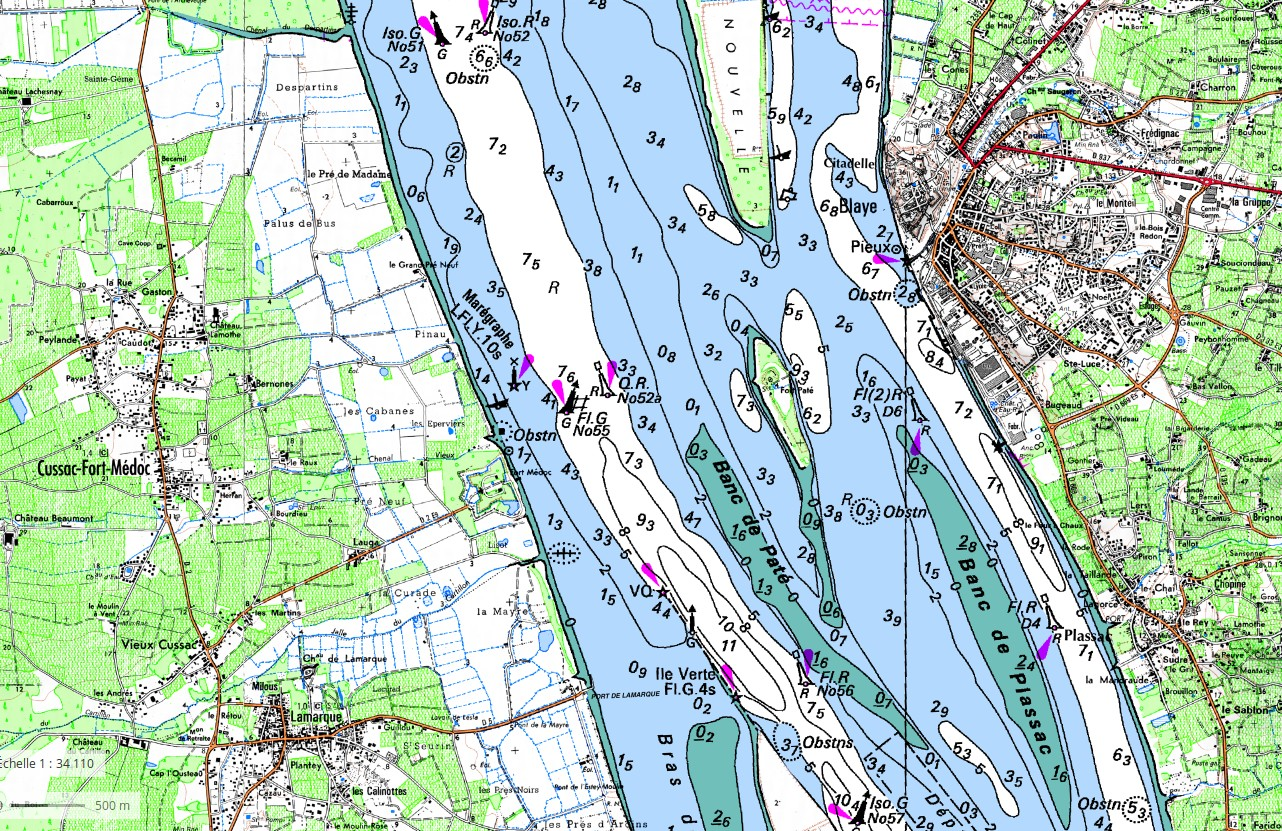
\includegraphics[width=10.5cm]{FortMedoc.jpg}
\end{figure}

\footnotesize
\textit{Sources: IGN and SHOM }
\normalsize

\end{frame}



% FRAME
\begin{frame}{Fields}

\textbf{What does this field represent ?}

\begin{figure}
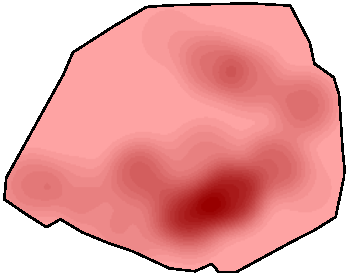
\includegraphics[width=7.5cm]{Champs.pdf}
\end{figure}

\end{frame}


%FRAME 
\begin{frame}{Field definition \& properties}
\begin{center}
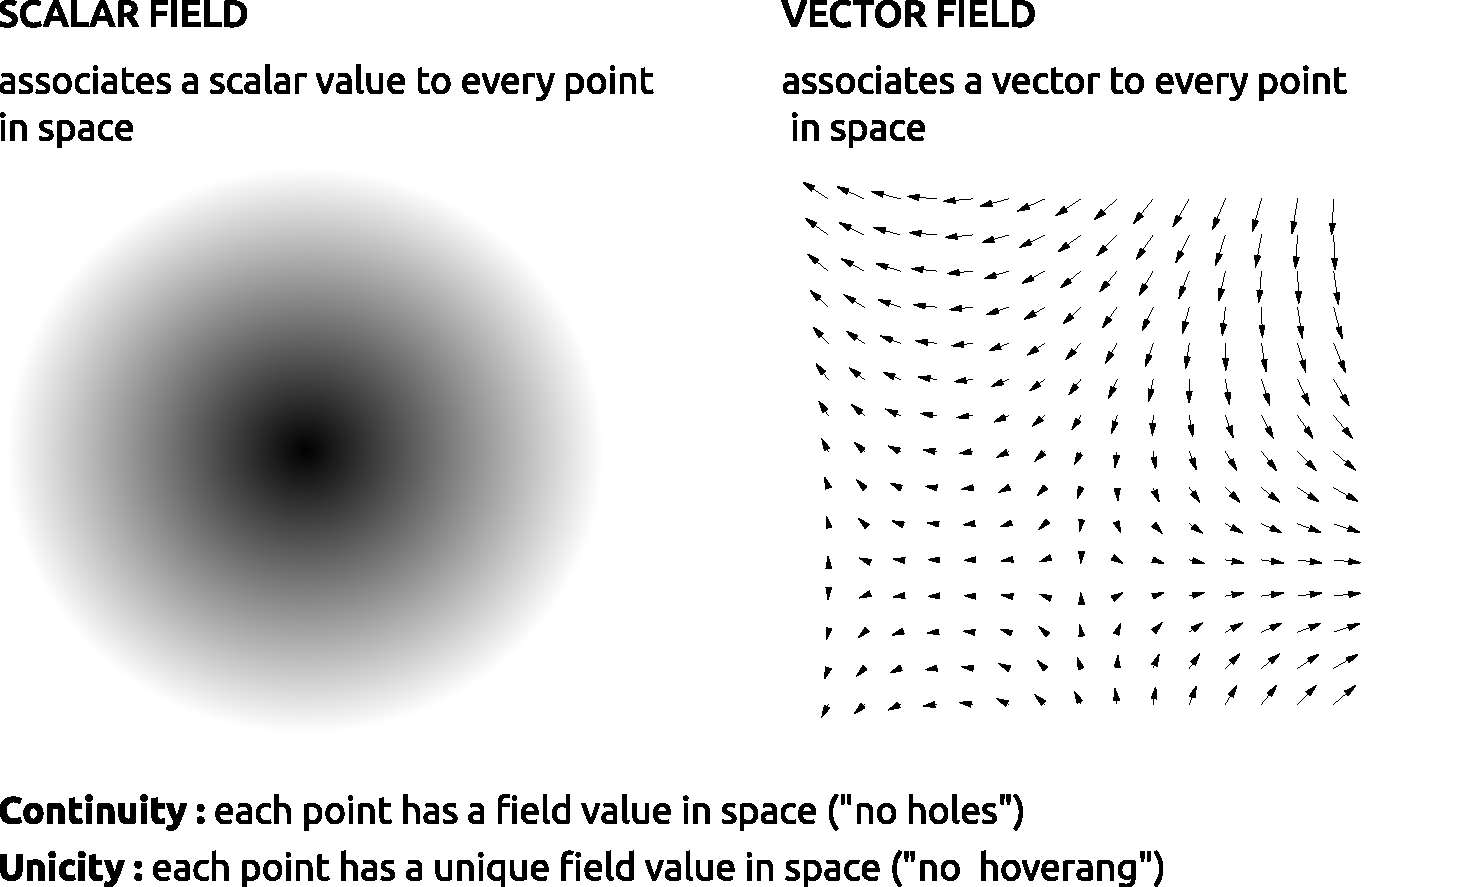
\includegraphics[width=10.5cm]{Champs_EN.pdf}
\end{center}
\end{frame}
% FRAME
\begin{frame}{Fields}

\textbf{Representation modes}

\begin{figure}
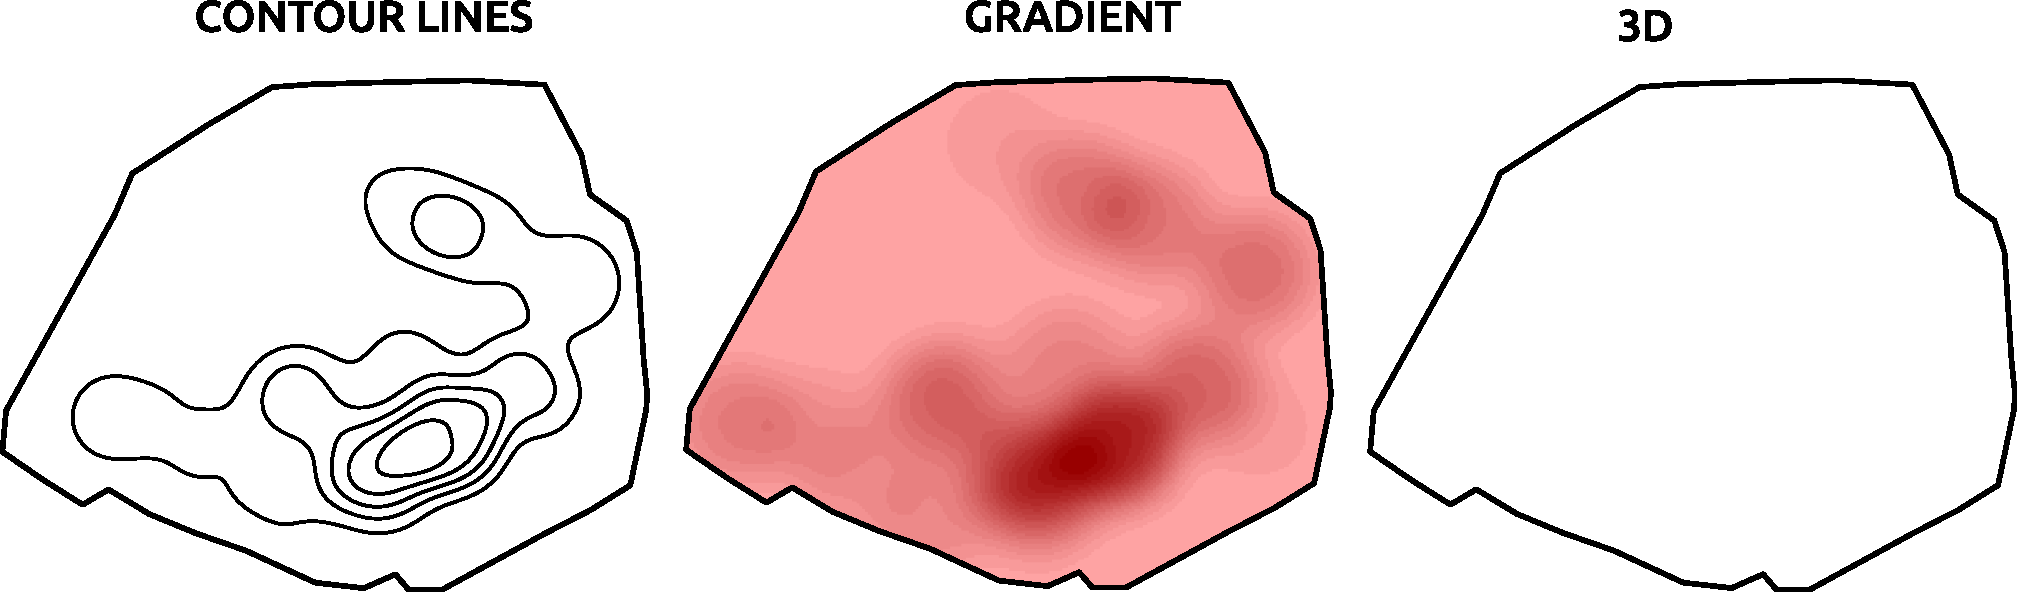
\includegraphics[width=10.5cm]{DeuxSorties_EN.pdf}
\end{figure}

\end{frame}



% FRAME
\begin{frame}{Fields}

\textbf{Representation modes examples}

\begin{figure}
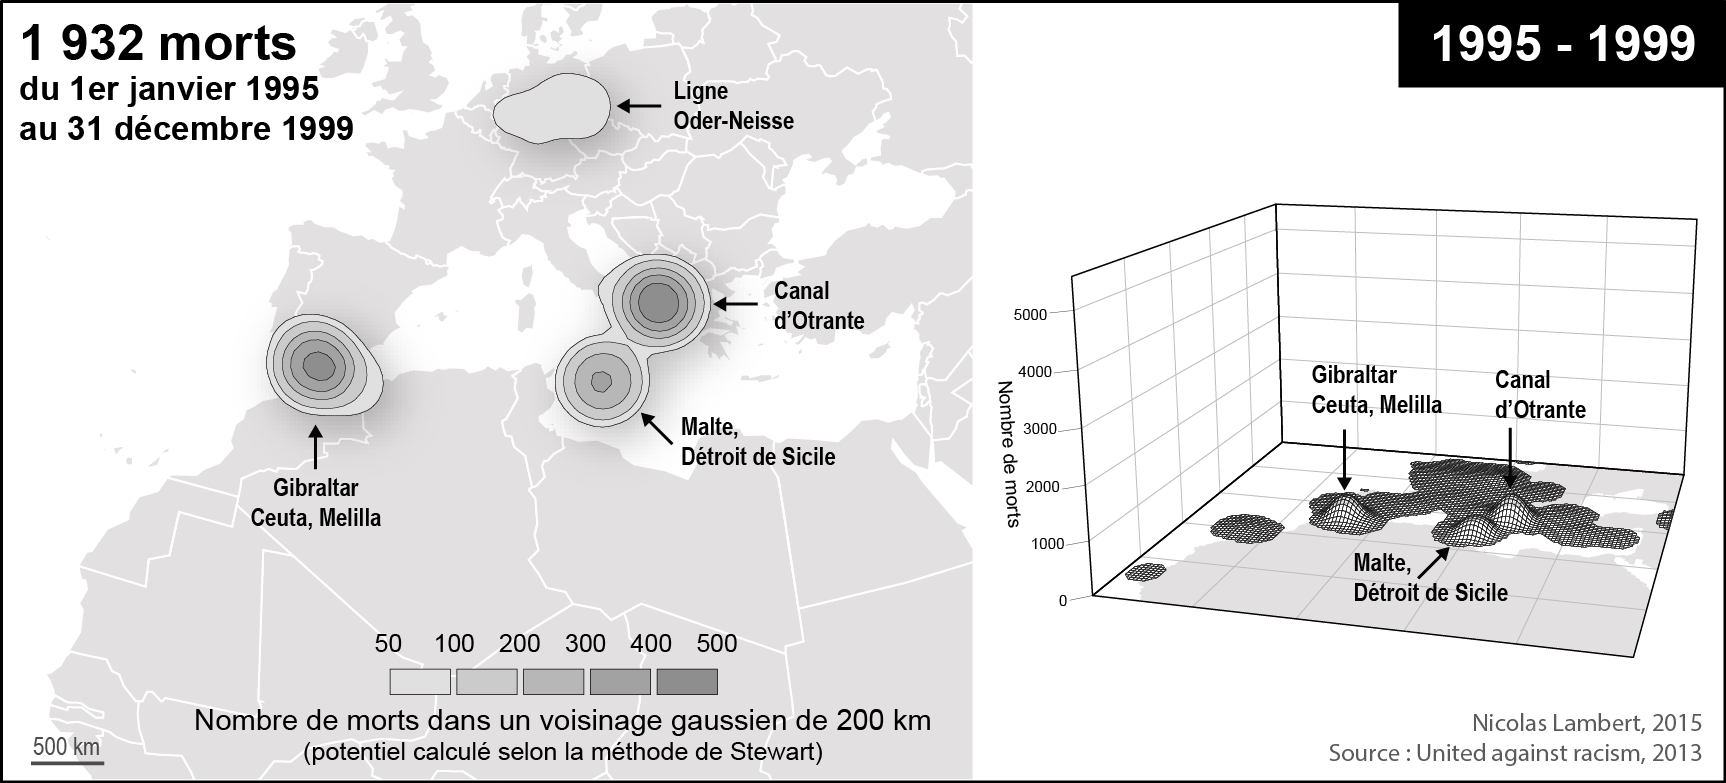
\includegraphics[width=11.5cm]{Migrants1.png}
\end{figure}

\end{frame}

% FRAME
\begin{frame}{Fields}

\textbf{Representation modes examples}

\begin{figure}
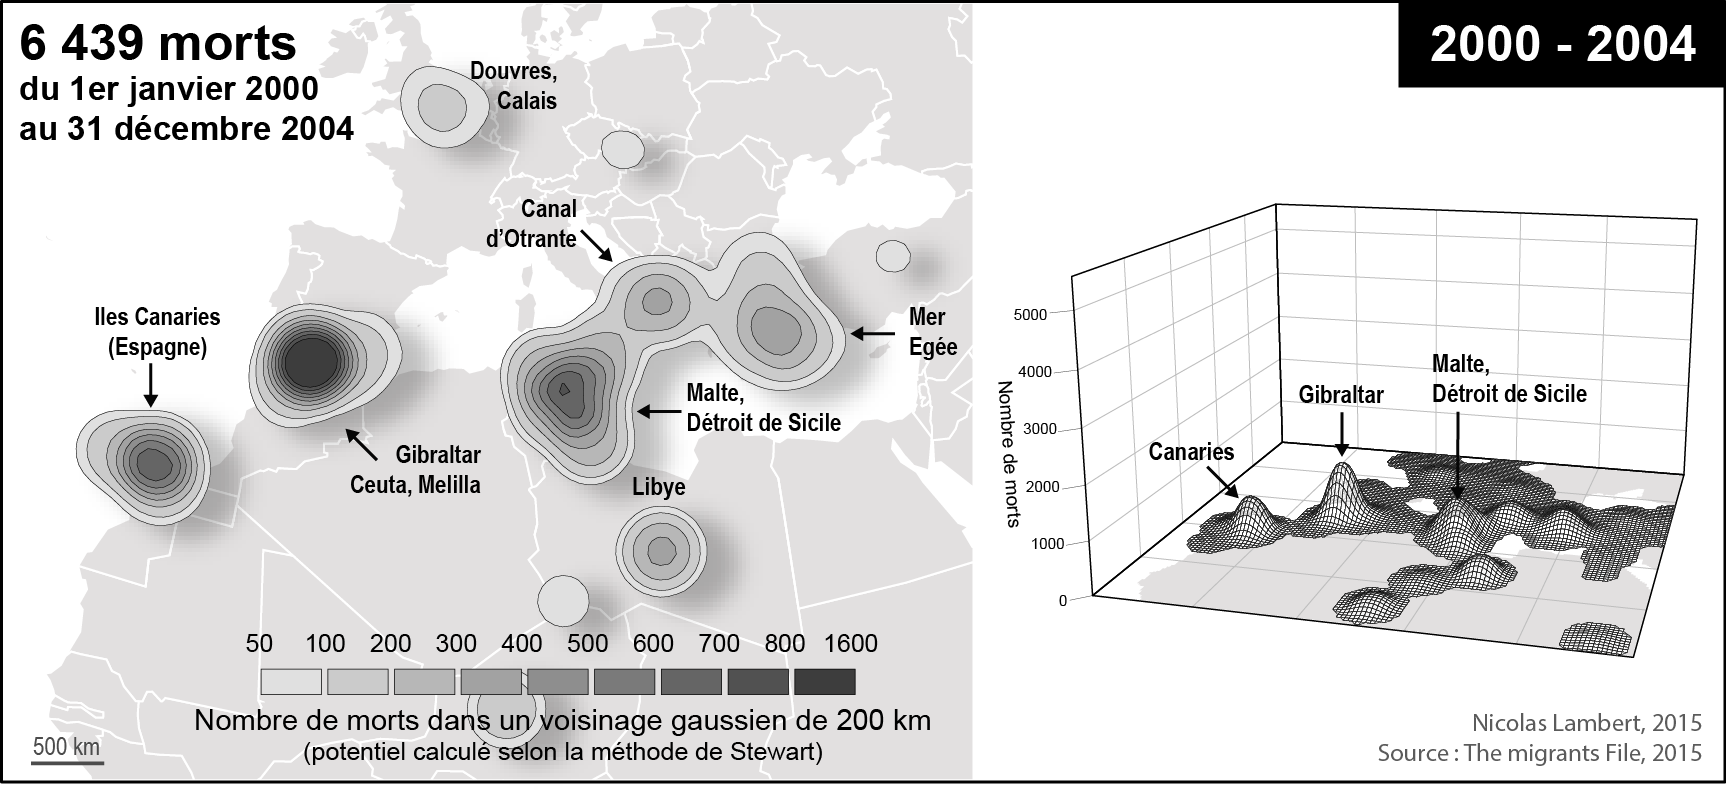
\includegraphics[width=11.5cm]{Migrants2.png}
\end{figure}

\end{frame}


% FRAME
\begin{frame}{Fields}

\textbf{Representation modes examples}

\begin{figure}
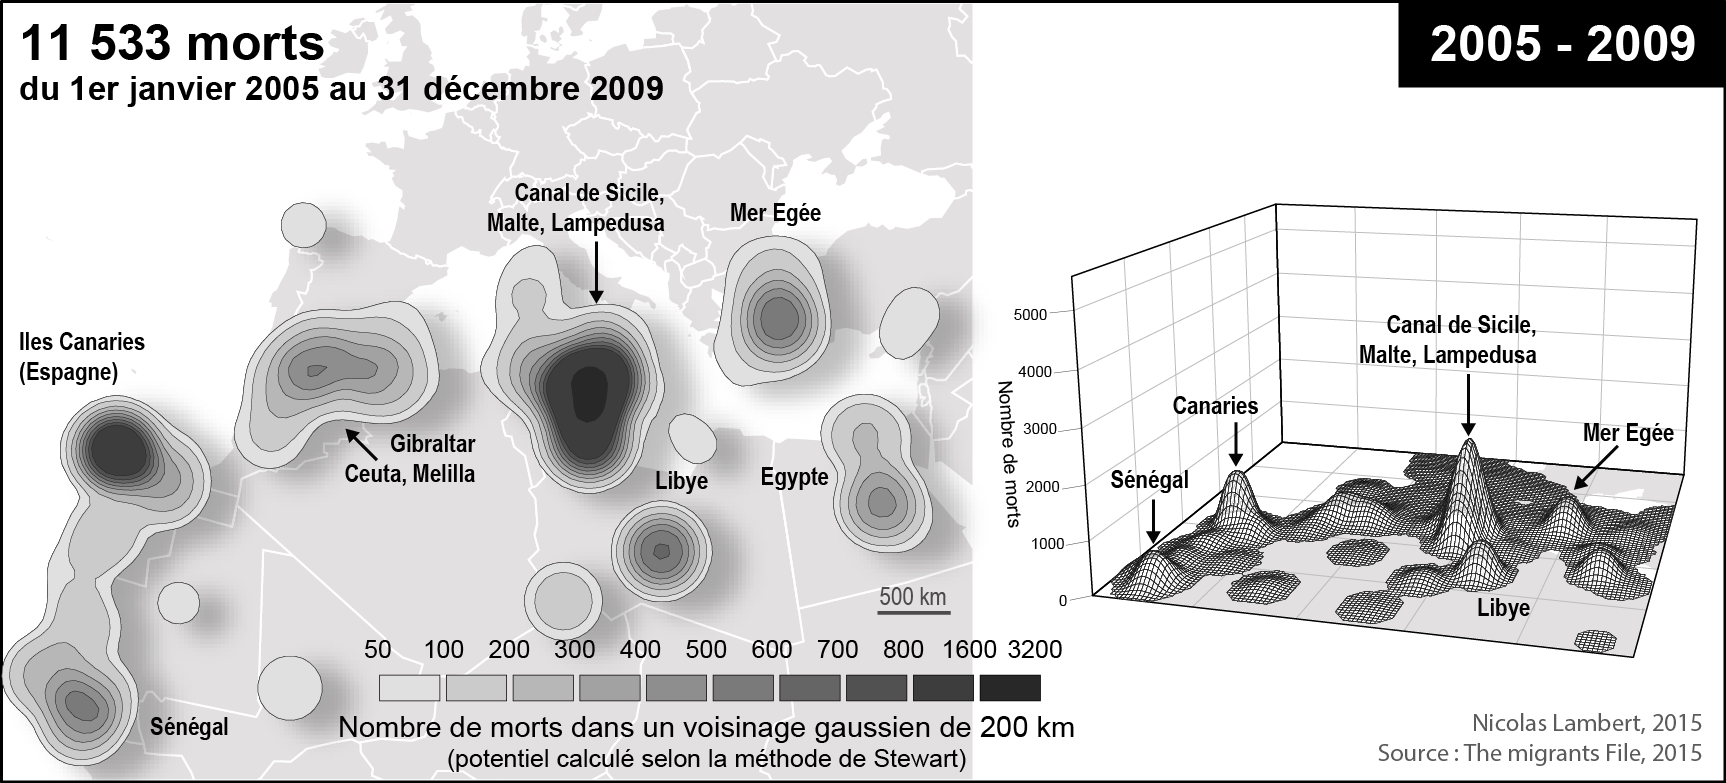
\includegraphics[width=11.5cm]{Migrants3.png}
\end{figure}

\end{frame}


% FRAME
\begin{frame}{Fields}

\textbf{Representation modes examples}

\begin{figure}
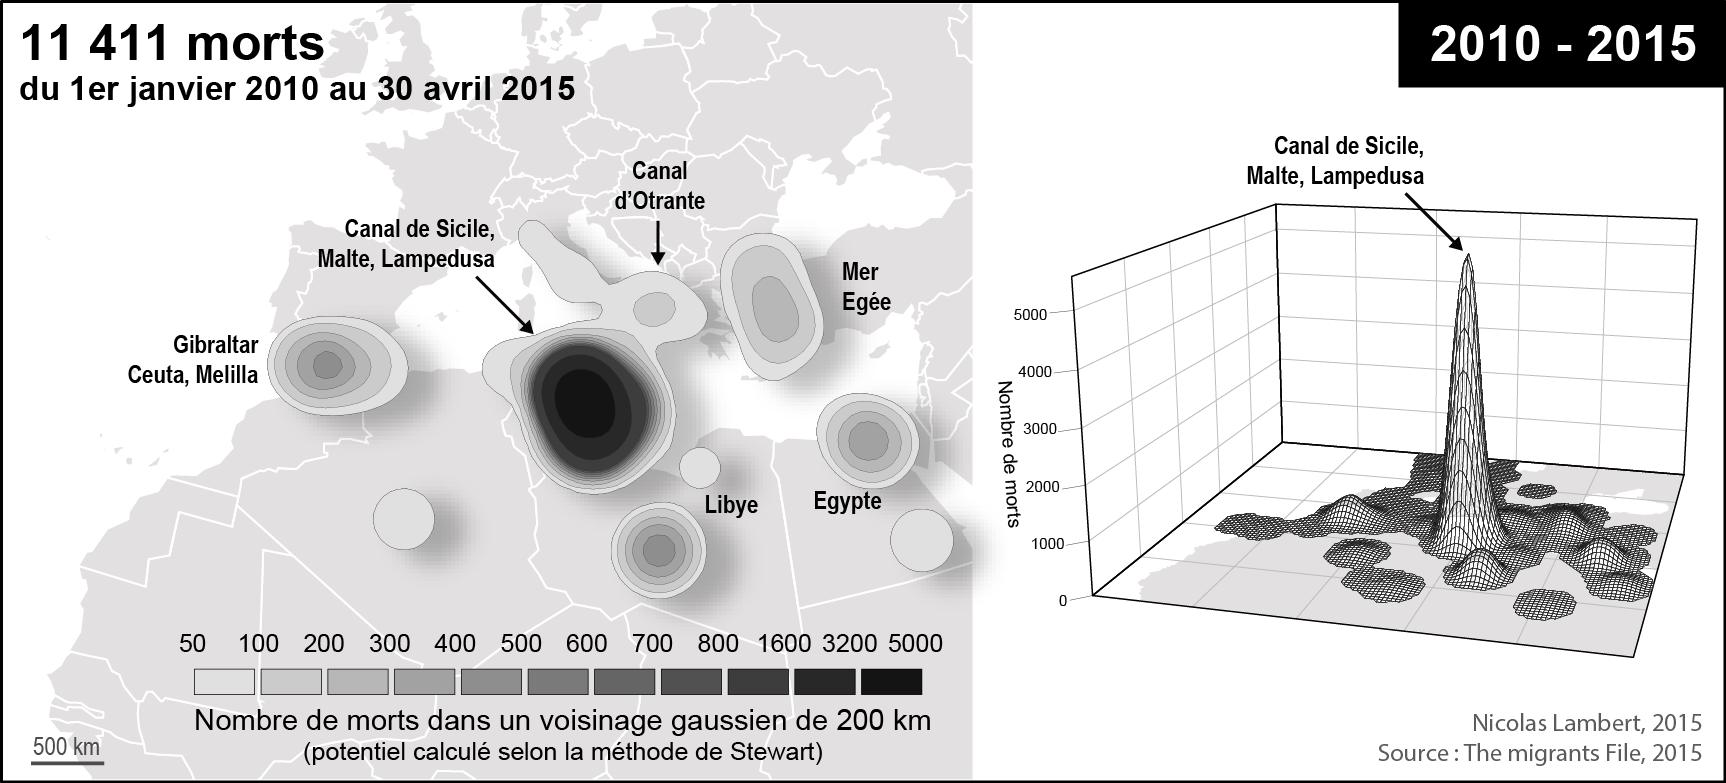
\includegraphics[width=11.5cm]{Migrants4.png}
\end{figure}

\end{frame}


% FRAME
\begin{frame}{Fields}

\begin{figure}
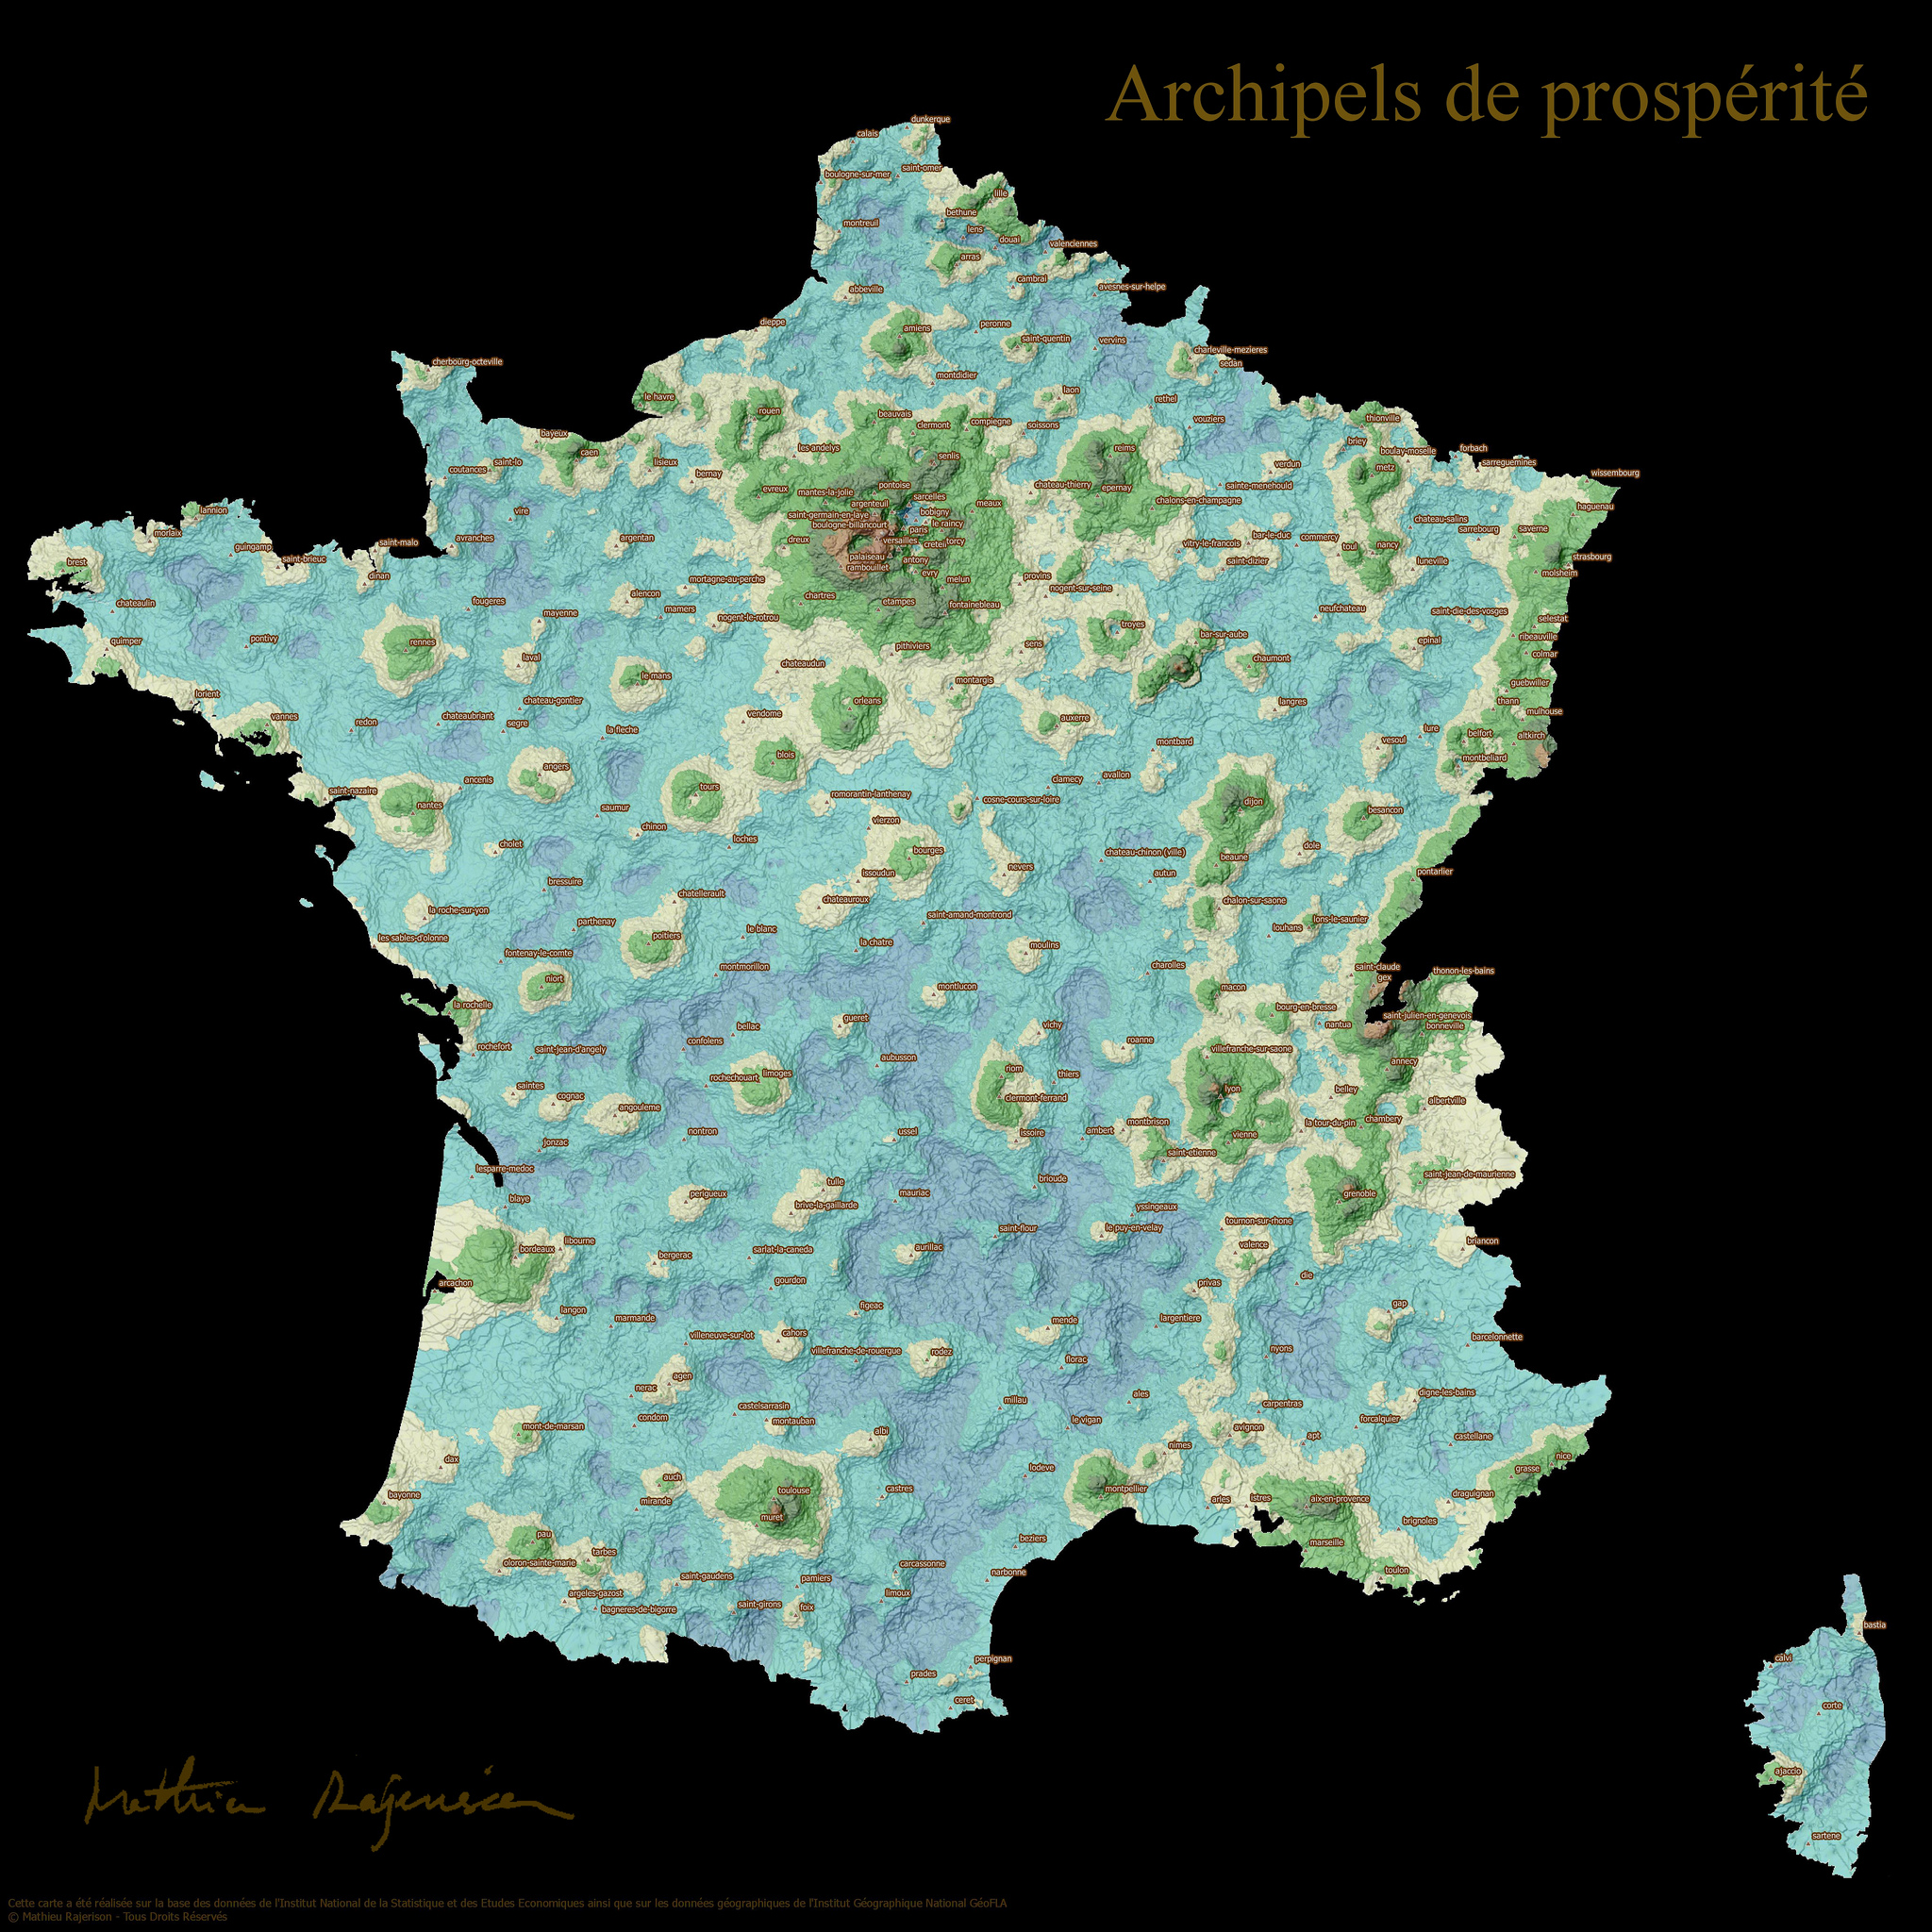
\includegraphics[width=7cm]{Rajerison_Revenu.jpg}
\end{figure}

\footnotesize
\textit{Source: Rajerison, Les archipels de la prospérité}
\normalsize

\end{frame}



% FRAME
\begin{frame}{Fields}

\begin{figure}
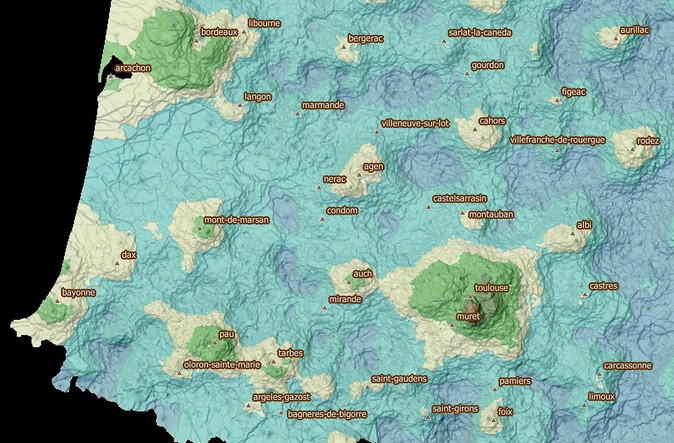
\includegraphics[width=9.5cm]{Rajerison_Zoom.jpg}
\end{figure}

\footnotesize
\textit{Source: Rajerison, Les archipels de la prospérité}
\normalsize
\end{frame}



% FRAME
\begin{frame}{Fields}
\begin{center}
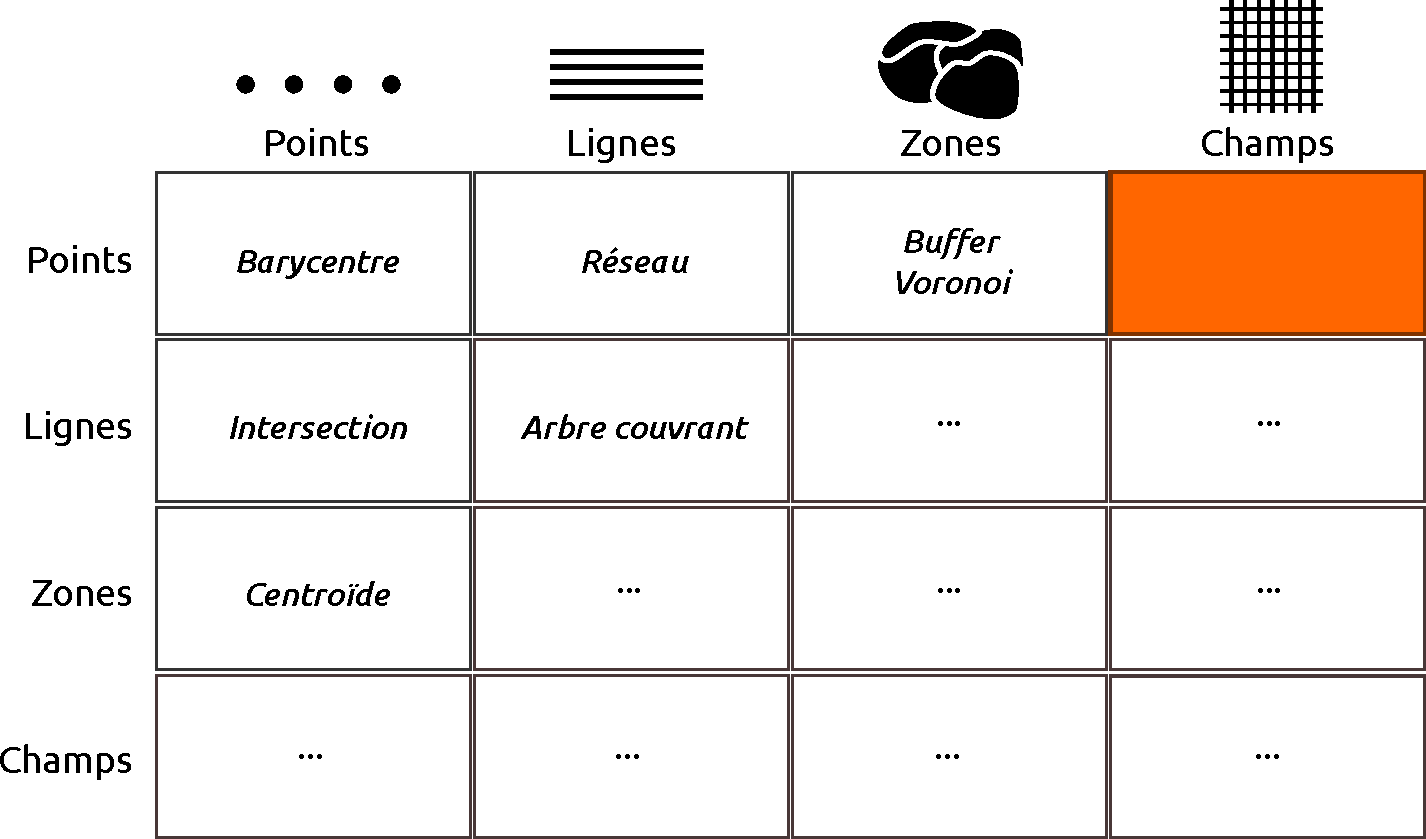
\includegraphics[width=10.5cm]{TypesObjets.pdf}
\end{center}
\end{frame}




